%%
%%       --- a chapter ---
%%
%% A chapter

\chapter[Sample Selection]{Long chapter heading} 
\label{ch:chapter2_label}

\section[Sec]{Section}
\label{sec:section2_label}
\section{Photometric Redshifts and Sample Selection}\label{sec:redshift}
Photometric redshifts for the entire source catalog were calculated using the EAZY photometric redshift software \citep{Anonymous:QJyxUpMF}. The fitting was done to all available bands using the default reduced template set based on the PEGASE spectral models of \citet{1997A&A...326..950F} with an additional template based on the spectrum of \citet{2010ApJ...719.1168E}. The additional template exhibits features expected in young galaxy populations such as strong optical emission lines and a high Lyman-$\alpha$ equivalent width.

For each galaxy we construct the full redshift probability distribution function (PDF), $P(z) \propto exp(-\chi_{z}^2/2)$, using the $\chi^2$-distribution returned by EAZY. 
Although EAZY allows the inclusion of a magnitude based prior when calculating redshifts, none was included in the fitting due to the large uncertainties still present in the H-band (our photometry selection band) luminosity function at high-redshifts \citep{Henriques:2012gs}.

\subsection{Selection Criteria} \label{sec:sample}
To investigate how the SMF evolves from $z =$ 4-7, we constructed a sample of galaxies in the redshift range $3.5 < z < 7.5$. To select a robust sample suitable for SED fitting, we apply a set of additional criteria based on the full redshift probability distribution for each galaxy to construct the different redshift samples, similar to those used in previous high-redshift sample selections \citep{2011MNRAS.418.2074M,Finkelstein:2012hr}. We then apply the following criteria:

%\begin{equation}(z_{sample}-0.5) < z_{phot} < (z_{sample}+0.5)
%\end{equation}

\begin{equation}\label{eq:crit1}
\int_{z_{sample}-0.5}^{z_{sample}+0.5} P(z)~dz > 0.4
\end{equation}

\begin{equation}\label{eq:crit2}
\int_{z_{peak}-0.5}^{z_{peak}+0.5} P(z)~dz > 0.6
\end{equation}
 
\begin{equation}\label{eq:crit3}
(\chi^{2}_{min} /N_{filters}-1) < 3
\end{equation}

\noindent where $z_{sample}$ = 4, 5, 6 and 7 for the respective bins and $z_{phot}$ is the redshift at the peak of the probability distribution (i.e. minimum $\chi^2$). 

The first criterion (Equation~\ref{eq:crit1}) requires that a significant amount of the probability distribution lies within the redshift range we are examining. The second criterion (Equation~\ref{eq:crit2}) requires that the bulk of the PDF lies close to the peak of the distribution, i.e. that the primary solution is a dominant one. Finally, we require that EAZY provides a reasonable fit (Equation~\ref{eq:crit3}). 

A signal to noise cut is placed on the J and H bands, requiring $\textup{SN}(J_{125}) > 3.5$ and $\textup{SN}(H_{160}) > 5$. Known AGN and sources with photometry flagged as effected by artefacts are removed. We also visually inspect each galaxy across all the HST bands, excluding sources which were caused or strongly affected by artefacts such as diffraction spikes, bright stars and image edges which were not excluded by any of the other criteria. 

Of the initial 34930 objects in the CANDELS GOODS South catalog, 3164 objects satisfy our first criterion. Of those objects, 256 are excluded by the second criterion and a further 167 are rejected based on their $\chi^{2}$. The signal to noise criteria exclude a further 274 sources and the remaining criteria exclude a further 176 sources. The resulting final sample comprises 2291 galaxies.

\begin{figure}
%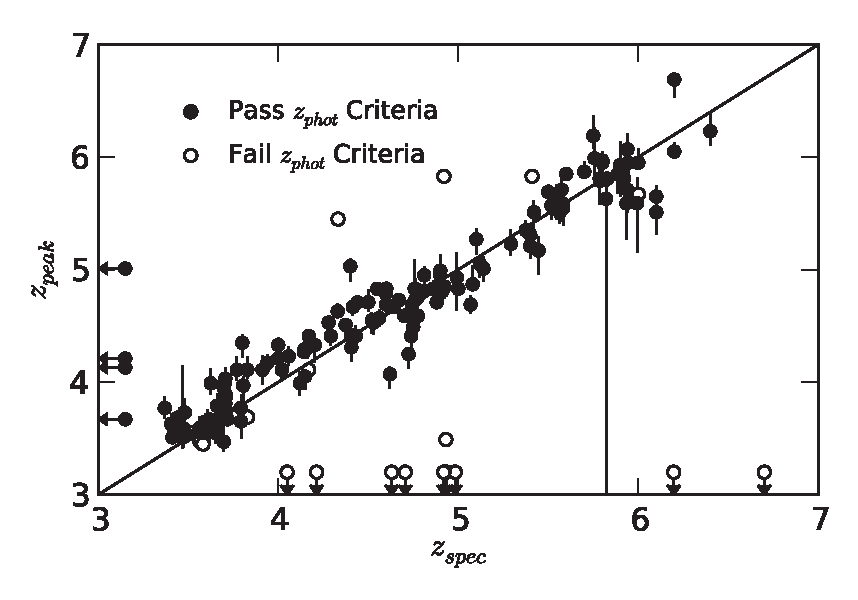
\includegraphics[width=84mm]{plots/fig1.eps}
\caption{Comparison between spectroscopic and photometric redshift for the galaxies in our sample with available spectroscopy and spectroscopic redshift quality of `Good" or better. The photometric redshift shown is the peak of the probability distribution ($\chi^2$ minimum) with 1-$\sigma$ lower and upper limits. Of the 11 galaxies classed as outliers, 6 are low-redshift interlopes at $z < 3$.}
\label{fig:specz}
\end{figure}

Figure~\ref{fig:specz} compares the available spectroscopic redshifts for the galaxies in our sample with the corresponding best-fit photometric redshift (minimum $\chi^2$) as found by EAZY. In total, there are 189 spectroscopic redshift matches for galaxies which pass our selection criteria and are therefore included in our samples. The matched spectroscopic redshifts are from the following surveys: \citet{LeFvre:2004ge,Stanway:2004gu,Vanzella:2008hp,Hathi:2008ca,Popesso:2009ht,Wuyts:2009gv,Rhoads:2009eb,Vanzella:2009ez,Balestra:2010bt,Kurk:2012ej} (\citet{Stark:2010hv} correct ref for Keck LBG spec-z's?).

We find that our redshift accuracy is good, with a scatter of just $\sigma_{z}/(1+z) = 0.038$ when outliers are excluded. We define outliers as $\left | \Delta z \right |/(1+z) > 0.15$, where $\Delta z =  (z_{spec}-z_{phot})$ \citep{Dahlen:2013eu}, and find an outlier fraction of 5.8\% (11 galaxies). This compares with \citet{2012ApJ...756..164F} who find a scatter of $\sigma_{z}/(1+z) = 0.044$  at $z > 3$ after excluding outliers (defined more strictly as $\left | \Delta z \right | > 0.5$) in the same CANDELS field. We also find that there is very little bias in our photometric redshifts, with $median(z_{spec}-z_{phot}) = 0.009$. Of the 11 galaxies classed as outliers, 6 lie at redshifts of $z < 3$ and are low-redshift interlopers which our selection criteria have not been able to exclude.

\citet{Dahlen:2013eu} have recently shown that by combining the results from multiple photometric redshift codes, the scatter and outlier fraction in photometric redshifts can be significantly reduced compared to the results of any single code. For the same set of 189 spectroscopic redshift sources, the photometric redshifts produced through the Bayesian combination outlined in \citet{Dahlen:2013eu} have $\sigma_{z}/(1+z) = 0.037$ with an identical outlier fraction of 5.8\% and $median(z_{spec}-z_{phot}) = 0.003$. 

Although utilising the photometric redshifts for the CANDELS GOODS-S field produced by this method would result in a small gain in photometric accuracy, we would no longer be able to reproduce the full selection method when running simulations. Given this small improvement, we are confident that the use of photometric redshifts produced by a single code will not adversely affect the overall accuracy of the results.

To investigate how the SMF evolves from z = 4-7, we then constructed four redshift samples in bins across this redshift range: $z \sim 4 ~(3.5 \leq z < 4.5)$, $z \sim 5~ (4.5 \leq z < 5.5)$, $z \sim 6~(5.5 \leq z < 6.5)$ and $z \sim 7 ~(6.5 \leq z < 7.5)$.

\subsection{Monte Carlo Samples}
Although we find that our photometric redshifts do well when compared with the matched spectroscopic redshifts, the group of outliers are indicative of the difficulties that exist in correctly distinguishing between the Lyman break of high-redshift galaxies at $z > 3$ and strong Balmer break galaxies at more moderate redshifts $z \approx 0.5-2.5$ in low S/N data. \citet{2012ApJ...748..122P,Pirzkal:2013ug} have shown that it is very difficult to categorically classify sources as high-redshift galaxies and not low-redshift interlopers using photo-z's or S/N criteria on the dropout bands.

Previous work using photometric redshifts has dealt with this problem by making use of the full redshift PDF when calculating luminosity functions \citep{2005ApJ...631..126D,2009MNRAS.395.2196M,2012arXiv1212.5222M}, thereby incorporating the uncertainty in the analysis. Due to the nature of the SED fitting code used for this work (described in Section~\ref{sec:masses}), the computational effort required to fit the mass at each redshift in order to integrate over the full PDF becomes impractical. As such, we chose to account for these problems in a different manner whilst still dealing with them in a straight-forward way. 

Rather than using only the best-fit redshift from our photometric analysis when selecting our sample, we instead draw the redshift for each galaxy randomly from its full PDF before placing it in the appropriate redshift sample. Where secure spectroscopic redshifts are available, we fix the redshift to that value for all samples (known interlopers are therefore excluded in all samples). This process was repeated 500 times to produce a set of samples to which we then apply the rest of the analysis described in the paper separately. We then average over the results from each sample, using the mean of this full set as our `true' value along with the 1-$\sigma$ upper and lower limits around this mean. 

\begin{table}
\caption{Average sample size and variance for each redshift bin for the 500 Monte Carlo samples generated, see text for details.}
\label{tab:samplesizes}
\begin{tabular}{@{}ccc}
\hline
 Redshift Bin & Mean Sample Size & Variance on sample size  \\
  \hline
 4 & 1235 & 180 \\
 5 & 416 & 63 \\
 6 & 169 & 25 \\
 7 & 42 & 9 \\
 \hline
\end{tabular}
\end{table}

The resulting sample sizes for each redshift bin are shown in Table~\ref{tab:samplesizes}. The varying samples account for both scattering between redshift bins for objects at the boundaries as well as objects moved out of the sample into secondary low-redshift solutions. The effect of this scattering into and out of the samples can be seen when comparing the combined mean samples sizes (1862) the our full high-redshift sample of 2291.

\begin{figure*}
%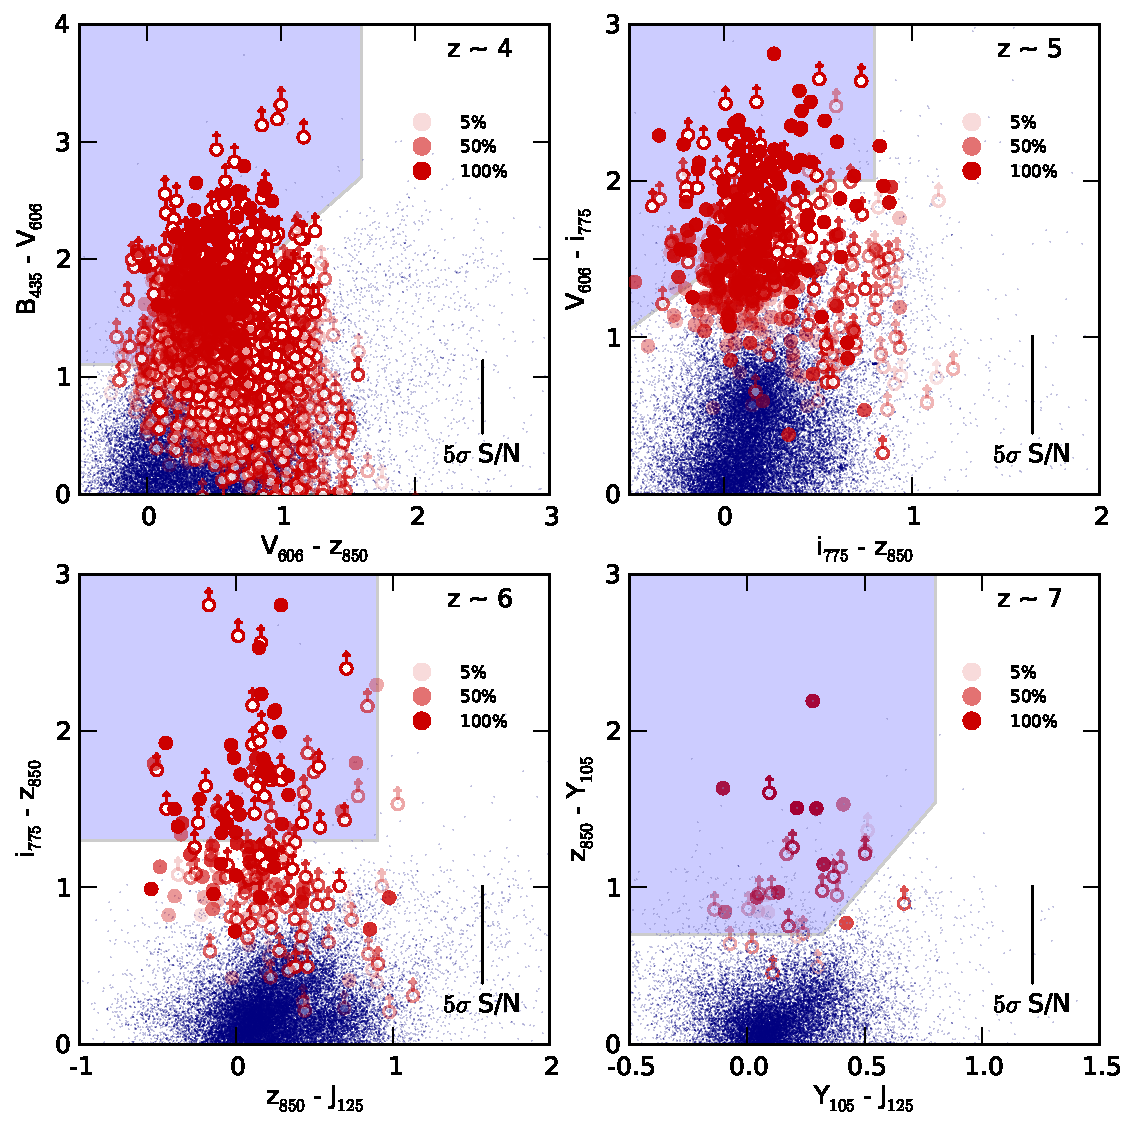
\includegraphics[width=140mm]{plots/fig2.eps}
\caption{The colours of our photometric redshift selected samples in relation to the two-colour cuts typically used to select Lyman break galaxies. Non-detections in a filter are converted to 2-$\sigma$ upper limits when calculating the colours. The shaded blue regions show the region in colour space used to select dropout galaxies in that redshift bin as described in  \citet{2007ApJ...670..928B}. Red symbols represent galaxies selected in our sample by our selection criteria, where the transparency of the symbols is determined by the number of Monte Carlo samples in which it is selected i.e. the fainter the symbol, the smaller the fraction of MC samples that galaxy is selected in. Example error bars corresponding to 5-$\sigma$ detections (for both filters in a given colour) are shown for each of the corresponding drop-out colours.}
\label{fig:colours}
\end{figure*}

The strength of using photometric redshifts for sample selection over colour cuts (especially when redshifts would still need to be calculated for a colour-cut sample in order to do SED fitting) is that the method can automatically make use of all available photometry. This is important because although photometric redshifts are still fitting primarily to the characteristic break at Lyman-$\alpha$ targeted by the colour selections, the filters long-ward of the break are useful in excluding low-redshift interlopers \citep{2011MNRAS.418.2074M}. Additionally, the large errors in colour possible due to low signal to noise and possible non-detections in the filter just short of the Lyman break means that likely high-redshift candidates can be scattered well outside the selection region when using colour cuts. 

Figure~\ref{fig:colours} shows the positions of our galaxy samples on the colour-colour planes commonly used to select dropout samples. It is obvious that many of the galaxies selected with photometric redshifts lie outside the selection regions (as taken from \citeauthor{2007ApJ...670..928B}~\citeyear{2007ApJ...670..928B}), especially those galaxies where colours must be calculated using an upper limit. To test whether the discrepancy between the observed colours and those expected for high-redshift galaxies can be explained solely by photometric scatter, we performed a range of tests on a mock catalog generated from the semi-analytic models of \citep{Somerville:2008ed}. Full details of these tests are outlined in Appendix~\ref{app:selection}, however our main findings are that the observed colours can be reproduced from intrinsic Lyman break-like colours and scattering proportional to the observed photometric errors. The agreement (or lack of) between dropout selections and photometric redshifts has also been investigated for GOODS-S specifically by \citet{2010ApJ...724..425D}.

Text of chapter.  

\subsection[Subsec]{Subsection}
\label{sec:subsec2_label}

\section{Selection method comparison}\label{app:selection}
Traditionally, (star-forming) galaxies at high-redshift have been selected using the Lyman break technique. Whereby galaxies are selected based on the observed colours across the redshifted Lyman break in their spectra.

When the observed colours of our photometric redshift selected galaxies are plotted in the same way, the selected galaxies span a range of colours far wider than those encompassed by the Lyman break selection criteria. Many of the galaxies have colours which would place them in the locus spanned by low-redshift galaxies, according to the Lyman break criteria. This has been observed before by \citet{2010ApJ...724..425D}, who find a similar range of colours for galaxies with photometric redshifts at $z \sim 4$ and 5.

This raises the question as to whether this discrepancy is solely due to photometric scatter in the relevant colours, if stellar populations different from those expected for the Lyman break criteria, or if in fact those galaxies outside the selection criteria are low-redshift interlopers or catastrophic failures in the photometric redshift estimation.

To answer these questions, we have taken a sample of galaxy mocks from the CANDELS semi-analytic models of \citet{Somerville:2008ed} across all redshifts, assigned photometric errors in each band based on the observed errors in the original catalog and then perturbed the flux by those errors. The resulting colours should then indicate the effects of photometric scattering on the intrinsic colours. We have assumed the errors are gaussian (the fluxes are perturbed by a value drawn from a gaussian where $\sigma =$ Flux Error) and have applied the errors based on the UDF, DEEP and WIDE regions. 

\begin{figure}
\centering
%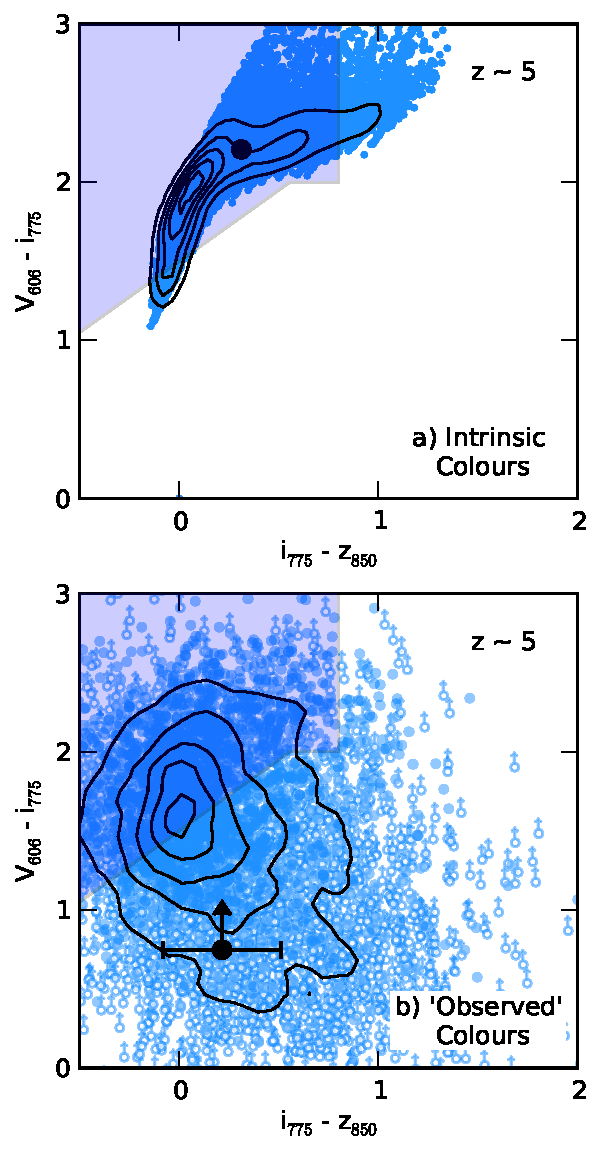
\includegraphics[width=80mm]{plots/figA1.eps}
\caption{Intrinsic colours of galaxies at $4.5 < z < 5.5$ from the CANDELS semi-analytic mock catalog. The colour coding corresponds to the apparent H$_{160}$ magnitude where blue = bright and red = faint. The background blue dots show the observed colours for the full CANDELS GOODS South catalog.}
\label{fig:mock_col}
\end{figure}

The intrinsic colours of the mock galaxies at $z \sim 5$ ($4.5 \leq z < 5.5$) are shown in Figure~\ref{fig:mock_col}. It is clear that the colours spanned by the galaxies lie well within the Lyman break selection criteria of \citet{2007ApJ...670..928B} and \citet{Gonzalez:2011dn}, with only a small fraction of galaxies redder than the criteria in the colour above the break or bluer across the Lyman break. Our input population therefore closely matches the colours for which the colour-colour criteria have been designed. The same is true across all redshift bins.

\begin{figure}
\centering
%\includegraphics[width=80mm]{plots/figA2.eps}
\caption{Observed colours of galaxies at $4.5 < z < 5.5$ from SAM mock sample after the photometry has been perturbed by flux errors proportional to the observed flux errors in the CANDELS DEEP region of observed photometry. The colour coding corresponds to the apparent H$_{160}$ magnitude (after perturbation by the error) where blue = bright and red = faint.}
\label{fig:mock_col_err}
\end{figure}

Figure~\ref{fig:mock_col_err} shows the colours of our mock galaxy catalog after being perturbed by errors drawn from the CANDELS DEEP region. Only galaxies with $SN(H_{160}) > 5$ are shown, matching the selection criteria for our high-redshift samples. The data points are also colour coded corresponded according to their observed $H_{160}$ magnitude (after error perturbation). It is immediately clear that photometric scatter pushes the colour spanning the Lyman break (the y-axis of each colour-colour plot) to values much lower values in $V_{606} - i_{775}$ than the range covered by the selection criteria. This is true across all regions, with the lower photometric error of the UDF (and part of the DEEP region for ACS bands) only differing in the faintness of those galaxies with the lowest signal to noise in the optical bands.

These simulations show that high-redshift galaxies can exhibit colours across the Lyman break well outside the traditional selection criteria. However, it is also important to show that the galaxies selected by photometric redshift with colours outside the colour criteria are indeed these high-redshift galaxies rather than lower redshift galaxies  in the same colour space.

\begin{figure}
\centering
%\includegraphics[width=80mm]{plots/figA3.eps}
\caption{Observed colours of galaxies from SAM mock sample selected as $z \sim 5$ by our photometric redshift method. Red circles correspond to input galaxies with an input redshift $4.5 < z < 5.5$, blue circles correspond to low-redshift interlopers incorrectly selected in the sample.}
\label{fig:mock_col_photz}
\end{figure}

In Figure~\ref{fig:mock_col_photz} we show the colours of galaxies with best-fitting photometric redshifts within the redshift bin of interest. Photometric redshifts have been calculated using the same method as described in Section 2. The selected galaxies span the full range of colours traced by the error perturbed colours of input high-redshift galaxies shown in the previous plots. Photometric redshift selection is therefore not as sensitive to photometric scatter across the Lyman break than the colour criteria for the same selection.

For redshifts $z = 4 - 5$, the majority of low-redshift interlopers which are selected as high-redshift exhibit colours outside of the colour criteria. However, the fraction of interlopers is very small compared to the number of 'real' high-redshift galaxies in this colour space. As redshift increases, the fraction of interlopers increases such that at $z \sim 7$ based on the best-fitting $z_{phot}$ alone, the fraction of outliers equals $\sim 0.60$, 0.51 and 0.72 for DEEP, UDF and WIDE respectively.

By applying additional cuts based on the full $P(z)$ distribution, the number of outliers can be reduced at the expense excluding some real sources. How strict the selection criteria are is a balance between minimising the contamination from interlopers and maximising the number of real high-redshift galaxies in the sample. Using the simulations however, we are able to correct the number densities for those real sources which are cut by our selection criteria.

For the selection criteria used in this work, the interloper fraction is reduced to an estimated 0.02, 0.07, 0.18 and 0.23 for $z \sim 4$, 5, 6 and 7 respectively. This was estimated by combining the fractions calculated for each field (assuming ERS to be comparable to DEEP) proportional to the number of high-redshift galaxies selected from each region of the field. In addition, by doing our analysis using the full redshift probability distribution as outlined in Section~\ref{sec:sample}, we account for this remaining fraction throughout our results.


Example reference in parentheses, (\citealt{ref1}).

Example reference list in parentheses, (\citealt{ref1,ref2}).



%% %% End of file...  %%
